\documentclass[12pt]{beamer}

\usepackage[size = custom, width = 92.71, height = 52.07, scale = 1.25]{beamerposter} % 36.5 in by 20.5 in

\usefonttheme{serif}

\usepackage[english]{babel}
\usepackage[utf8x]{inputenc}
\usepackage[T1]{fontenc}
\usepackage{lmodern}
\usepackage{indentfirst}
\usepackage{ragged2e}
\usepackage[]{natbib} 
\usepackage{graphicx}
\usepackage{animate}
\usepackage{color}
\usepackage{tikz}
\usepackage{colortbl}
\usetikzlibrary{arrows.meta}
\tikzset{>={Latex[width=5mm,length=5mm]}}


\usepackage{tcolorbox}


% For 'InkScape' integration
\usepackage{import}
\usepackage{xifthen}
\usepackage{pdfpages}
\usepackage{transparent}


\setbeamertemplate{navigation symbols}{}
\setbeamertemplate{caption}[numbered]

\definecolor{custom-bg}{RGB}{198, 217, 241}
\definecolor{custom-bd}{RGB}{55, 93, 138}
\definecolor{strong-blue}{RGB}{1, 43, 91}


\setbeamercolor{block title}{fg = red, bg = red}
\setbeamercolor{header-color}{fg = strong-blue, bg = white}
\setbeamercolor{background canvas}{bg = custom-bg}

%%% blocks
\defbeamertemplateparent{blocks}[framed]{block begin,block end}[1][]
{[#1]}

\defbeamertemplate{block begin}{framed}[1][]
{
	\begin{tcolorbox}[%
		colback=white,%
		colframe=custom-bd, arc=5mm]%
		{\vskip\smallskipamount%
			\raggedright\usebeamerfont*{block title}%
			\usebeamercolor[fg]{title}\insertblocktitle}%
		\vskip\smallskipamount%
		\raggedright%
		\usebeamerfont{block body}%
	}
	
	\defbeamertemplate{block end}{framed}[1][] {\end{tcolorbox}}

\setbeamertemplate{blocks}[framed]


\begin{document}
	\begin{frame}[t]
		\vspace{-46pt}
		\begin{columns}[t]
			\begin{column}{1\textwidth} \justifying % HEADER
				\begin{block}

					\begin{columns}[T]
						\begin{column}{0.2\textwidth}
							
\includegraphics[width=1.15\linewidth]{Images/KAUST_logo} 
						\end{column}
						\begin{column}{0.67\textwidth}
							\vspace{32pt}
							\begin{beamercolorbox}[wd=1.00\textwidth]{header-color}	
								{\Large \textcolor{strong-blue}{{Integrating Compartment and Point Process Models for Spatio-Temporal Modeling of Infectious Diseases}} \par} \vspace{12pt}
								
								{\normalsize \textcolor{black}{
									André Victor Ribeiro Amaral${\phantom{|}}^{1, \star}$, 
									Jonatan A. González${\phantom{|}}^{1}$,
									Paula Moraga${\phantom{|}}^{1}$
								}}	\vspace{16pt}
								
								{\footnotesize \textcolor{black}{
									${}^{1}\hspace{8pt}$Computer, Electrical and Mathematical Sciences and Engineering Division, King Abdullah University of Science and Technology (KAUST).  \\ \vspace{3pt}
									${}^{\star}$ E-mail: \texttt{andre.ribeiroamaral@kaust.edu.sa}
								}}
							\end{beamercolorbox}
							\vspace{24pt}
						\end{column}
						\begin{column}{0.13\textwidth}
							\vspace{20pt}
							
\includegraphics[width=0.9\linewidth]{Images/JSM_logo}
						\end{column}
					\end{columns}
					
				\end{block}
			\end{column}
		\end{columns}
		
		
		\vspace{-4pt}
		\begin{columns}[t]
			%======================================== FIRST COLUMN ========================================
			\begin{column}{0.24175\textwidth} \justifying % FIRST COLUMN
				
			\begin{block}{}
			\textcolor{strong-blue}{\Large 1. Objective} \justifying \vspace{12pt}
		
			We are interested in modeling the infected individuals in space and time. To do this, we will \vspace{6pt}
			
			\begin{enumerate}
				\justifying
				\item Fit a temporal (compartment) model, and
				\item Use the previous step acquired information as the mean of a LGCP for the point pattern representing the infected individuals in the studied region and time interval.
			\end{enumerate}
		
			\begin{figure}[!ht]
				\centering
				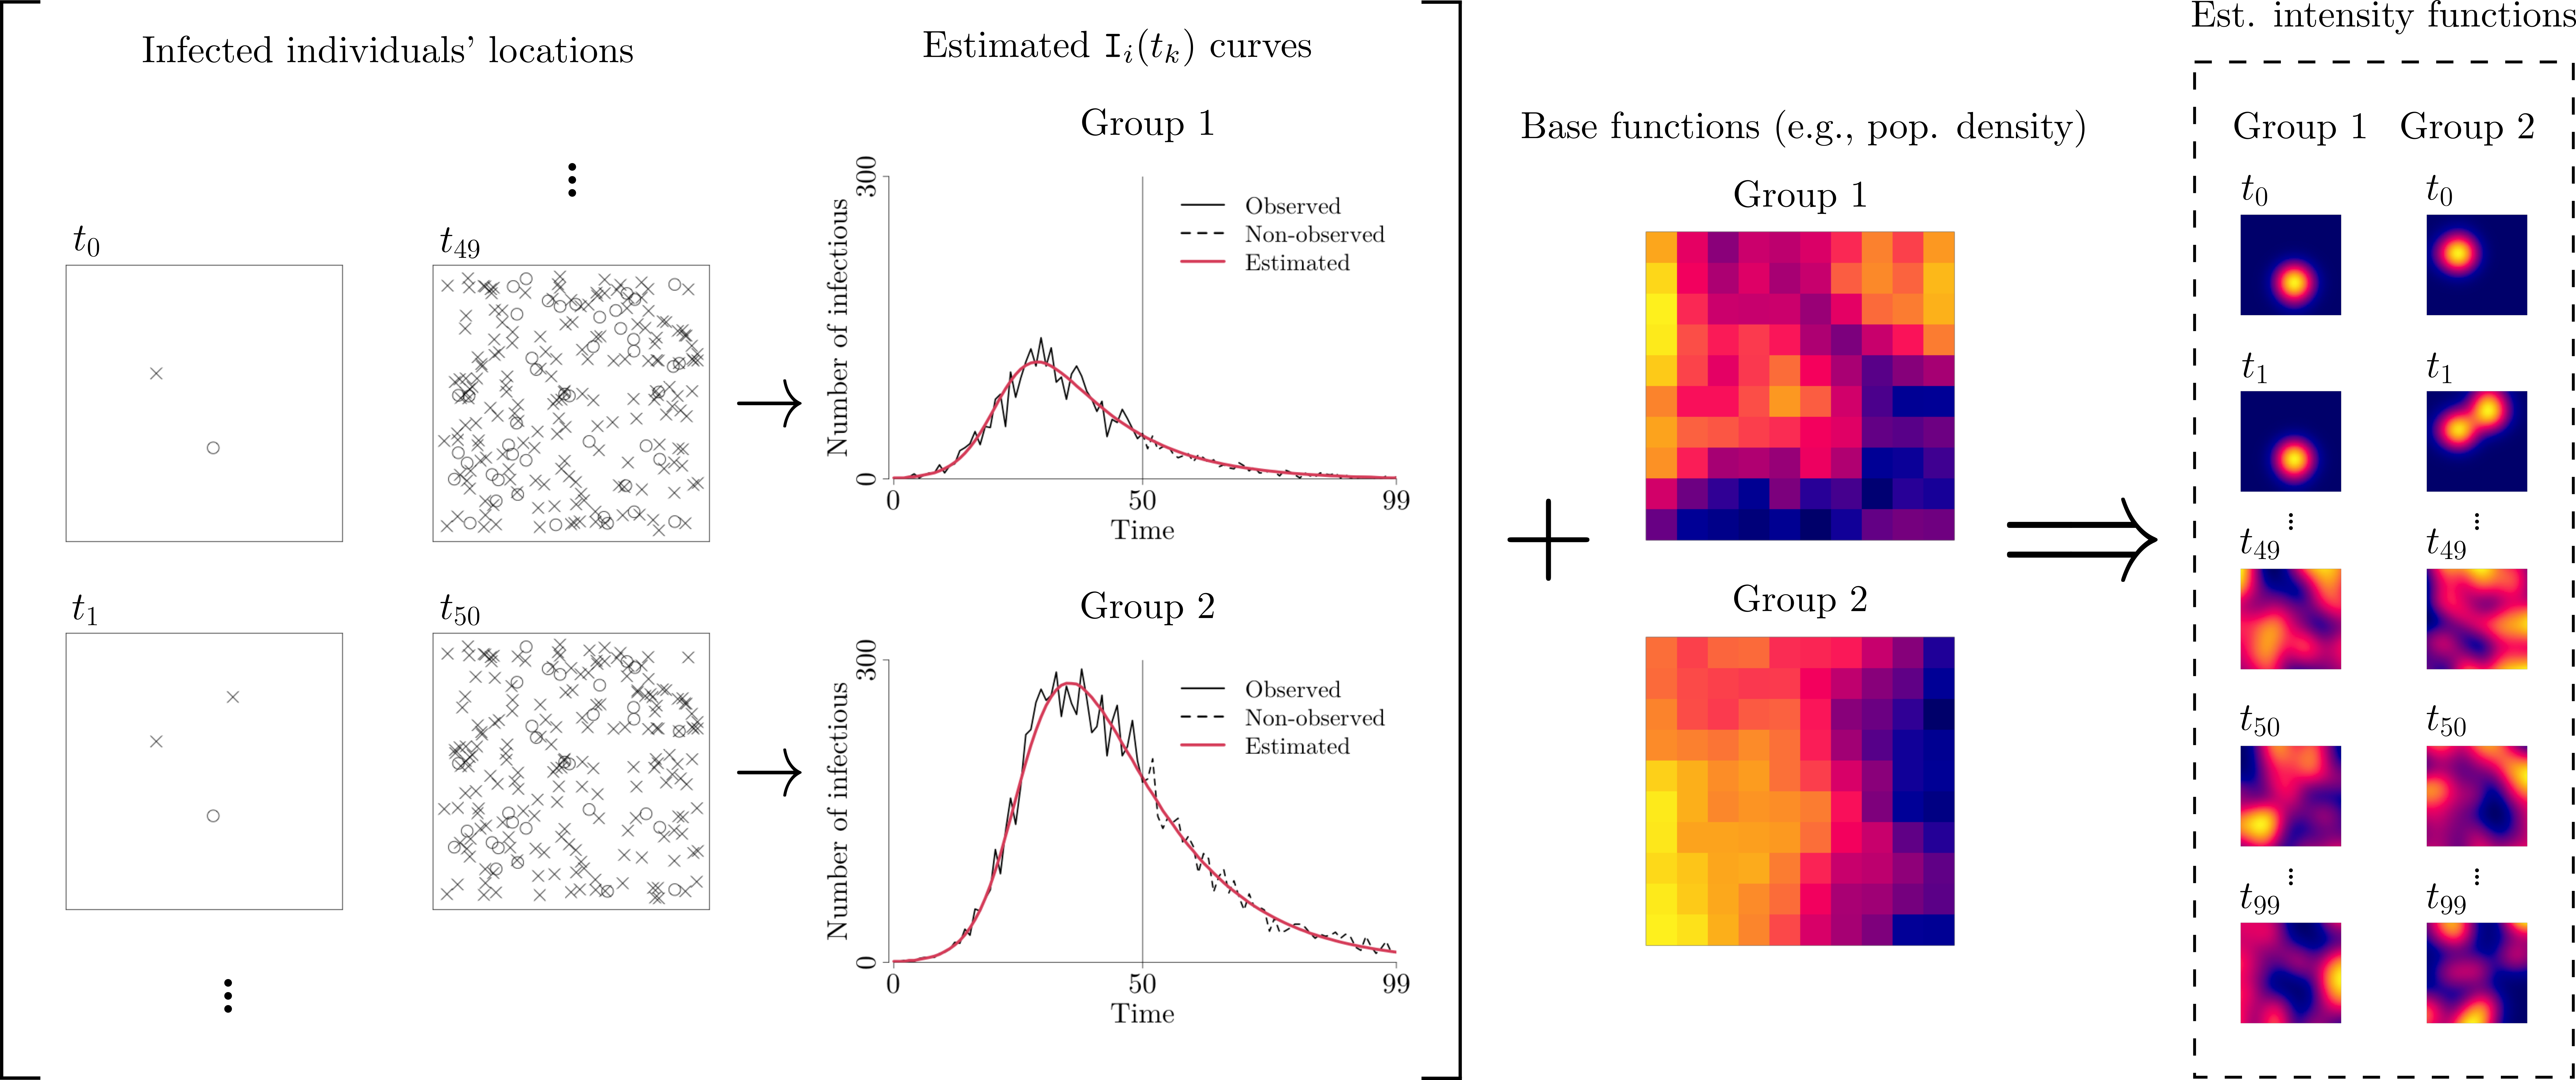
\includegraphics[width = 1\textwidth]{Images/diagram.png}\vspace{-6pt}
				\caption{\justifying Two-step spatio-temporal modeling approach.}
				\label{fig:diagram}
			\end{figure}
		
			\textcolor{strong-blue}{\Large 2. \texttt{SIR} modeling} \justifying \vspace{12pt}

			The base-\texttt{SIR} model \citep{kermack1927contribution} is described as follows\vspace{-15pt}
			\begin{figure}[!ht]
				\begin{tikzpicture}
					\centering
					\draw[draw=black] (0, 0) rectangle ++(5.5, 1.5);
					\draw[draw=black] (7.5, 0) rectangle ++(5.5, 1.5);
					\draw[draw=black] (15, 0) rectangle ++(5.5, 1.5);
					\draw[->](5.5, 0.75) -- (7.5, 0.75);
					\draw[->](13, 0.75) -- (15, 0.75);
					\node[] at (2.75, 0.75) {Susceptible};
					\node[] at (10.25, 0.75) {Infected};
					\node[] at (17.75, 0.75) {Recovered};
					\node[] at (6.5, 2.25) {\footnotesize Transmission};
					\node[] at (14, 2.25) {\footnotesize Recovery};
				\end{tikzpicture}
			\end{figure}
			and it has the following assumptions \vspace{6pt}
			\begin{enumerate}
				\item Homogeneous population with uniform mixing.
				\item Constant infectious and recovery rates.
				\item Preserved population mass.
			\end{enumerate}
			
			Such a model can be extended in different ways.
			
			\vspace{2pt}
			\end{block}
		
			
			\end{column}
		
			%======================================== SECOND COLUMN ========================================
			\begin{column}{0.24175\textwidth} \justifying % SECOND COLUMN
			
			\begin{block}{}
			\justifying
			
			Let $\texttt{S}_i(t)$, $\texttt{I}_i(t)$, and $\texttt{R}_i(t)$ denote the number of susceptible, infected, \hspace{-1pt}and recovered individuals, \hspace{-1pt}respectively,\hspace{-1pt} at time \hspace{-1pt}$t$ for age-group $i$. Then,
			\begin{align} \label{eq:SIRmodel}
				\frac{d\texttt{S}_i(t)}{dt} &= -\beta \texttt{S}_i(t) \, \displaystyle\raisebox{-18pt}{\scalebox{3.2}{\ensuremath{\sum}}}_{\text{all}\,j}C_{ij}\cdot\frac{\texttt{I}_j(t)}{\texttt{N}_j} \\
				\frac{d\texttt{I}_i(t)}{dt} &= +\beta \texttt{S}_i(t) \, \displaystyle\raisebox{-18pt}{\scalebox{3.2}{\ensuremath{\sum}}}_{\text{all}\,j}C_{ij}\cdot\frac{\texttt{I}_j(t)}{\texttt{N}_j} - \gamma \texttt{I}_i(t) \nonumber \\
				\frac{d\texttt{R}_i(t)}{dt} &= +\gamma \texttt{I}_i(t), \nonumber
			\end{align}
			such that $C_{ij}$ is a contact matrix, $\texttt{N}_i(t) = \texttt{N}_i$, $\forall t$, and $\beta, \gamma > 0$.  We will define a solution at $\{t_k\}_k$.
			
			\vspace{18pt}
			
			\textcolor{strong-blue}{\Large 3. Point Process modeling} \justifying \vspace{12pt}
			
			Let $\xi(t_k)$ be a log-Gaussian Cox process driven by $\Lambda(\mathbf{u}; t_k)$. In particular,
			\begin{align} \label{eq:llambda}
				\Lambda(\mathbf{u}; t_k) = \mu(\mathbf{u}; t_k) \cdot \exp\{\zeta(\mathbf{u}; t_k)\},
			\end{align}
			where  $\zeta(\mathbf{u}; t_k)$ is a stationary Gaussian process with constant mean function given by $-\sigma^2/2$, and $\text{Cov}(\zeta(\mathbf{u}_1; t_k), \zeta(\mathbf{u}_2; t_k)) = \sigma^2 \rho(h; t_k)$. \vspace{12pt}
			
			Specific choices of $\mu(\mathbf{u}; t_k)$ were discussed by \cite{diggle2006spatio}.
			
			\vspace{18pt}
			
			\textcolor{strong-blue}{\Large 4. Temporal modeling (practical)}\justifying\vspace{12pt}
			
			For a set of initial values  $(\texttt{S}_i(0), \texttt{I}_i(0), \texttt{R}_i(0))$, $\forall i$, and initial guesses for $\beta$ and $\gamma$, we can solve the system of ODEs for $\texttt{S}_i(t_k)$, $\texttt{I}_i(t_k)$, and $\texttt{R}_i(t_k)$ with a numerical method. We will name solutions $\texttt{S}_i^{\texttt{ODE}}(t_k)$, $\texttt{I}_i^{\texttt{ODE}}(t_k)$, and $\texttt{R}_i^{\texttt{ODE}}(t_k)$. 
			
			\vspace{33pt}
			\end{block}

			\end{column}
		
			%======================================== THIRD COLUMN ========================================
			\begin{column}{0.24175\textwidth} \justifying % THIRD COLUMN
		
			\begin{block}{}
			\justifying
			
			Now, suppose that we have obtained $\texttt{i}_i(t_k)$, $\forall i, k$. One way to model such data is assuming that they come from a certain probability distribution with mean given by the ODE solution $\texttt{I}_i^{\texttt{ODE}}(t_k)$. In particular, 
			\begin{align} \label{eq:InfNB}
				\texttt{I}_i(t_k) \sim \text{Negative Binomial}(\texttt{I}_{i}^{\texttt{ODE}}(t_k), \varphi),
			\end{align}
			such that $\varphi$ is the overdispersion parameter. \vspace{12pt}
			
			In that way, we will have to\vspace{6pt}
			\begin{enumerate}
				\justifying
				\item Set initial values for $\beta$, $\gamma$, and $\varphi$.
				\item Solve Model \eqref{eq:SIRmodel} for $\texttt{S}_i(t_k)$, $\texttt{I}_i(t_k)$, and $\texttt{R}_i(t_k)$.
				\item Plug the $\texttt{I}_i^{\texttt{ODE}}(t_k)$ curve into the mean component of Model \eqref{eq:InfNB} and evaluate it.
				\item Update $\beta$, $\gamma$, and $\varphi$, and get back to (2.) until reach convergence.
			\end{enumerate}
			
			Here, we used \texttt{RStan} \citep{rstanpackage} to estimate the posterior distribution of $\boldsymbol{\theta} = (\beta, \gamma, \varphi)^{\top}$.
			
			\vspace{18pt}
			
			\textcolor{strong-blue}{\Large 5. ST modeling (practical)}\justifying\vspace{12pt}
			
			The final model is specified as follows
			{\footnotesize
			\begin{align} \label{eq:modelSpatioTemporal}
				\text{N}_i(t_k)|\Lambda_i(\mathbf{u}; t_k) = \lambda_i(\mathbf{u}; t_k) &\sim \text{Poisson}\left(\int_{\hspace{3pt}\mathcal{U}}\lambda_i(\mathbf{u}; t_k)d\mathbf{u}\right), ~\forall i, k \\
				\Lambda_i(\mathbf{u}; t_k) &= \mu_i(\mathbf{u}; t_k) \cdot \exp\{\zeta_i({\mathbf{u}; t_k})\} \nonumber \\
				\mu_i(\mathbf{u}; t_k) &= \lambda_{0, i}(\mathbf{u}; t_k) \cdot \texttt{I}_i(t_k) \nonumber \\ 
				\zeta_i(\mathbf{u}; t_k | \boldsymbol{\eta}_i) &\sim \text{Gaussian Process} (\beta_{0, i}, \phi_i(h; t_k | \boldsymbol{\eta}_i)) \nonumber \\
				\boldsymbol{\eta}_i &\sim \text{priors}, \nonumber
			\end{align}
			}%
			such that $\phi_i(h; t_k | \boldsymbol{\eta}_i)$ is a covariance function, and $\boldsymbol{\eta}_i$ is the vector of parameters.\vspace{6pt}
			
			Finally, Model \eqref{eq:modelSpatioTemporal}  was fitted using \texttt{R-INLA} \citep{rue2009approximate}. 
			
			\vspace{31pt}
			
			\end{block}

					
			\end{column}
		
			%======================================== FOURTH COLUMN ========================================
			\begin{column}{0.24175\textwidth} \justifying % THIRD COLUMN
								
				\begin{block}{}
				\textcolor{strong-blue}{\Large 6. Case Study}\justifying\vspace{12pt}
				
				We consider as a study region an area of approx. 3 km${}^{2}$ in São Paulo, Brazil. Then, we divided people into three age groups: 0--19, 20--59, 60+.
				
				\begin{figure}[!ht]
					\centering\vspace{-3pt}
					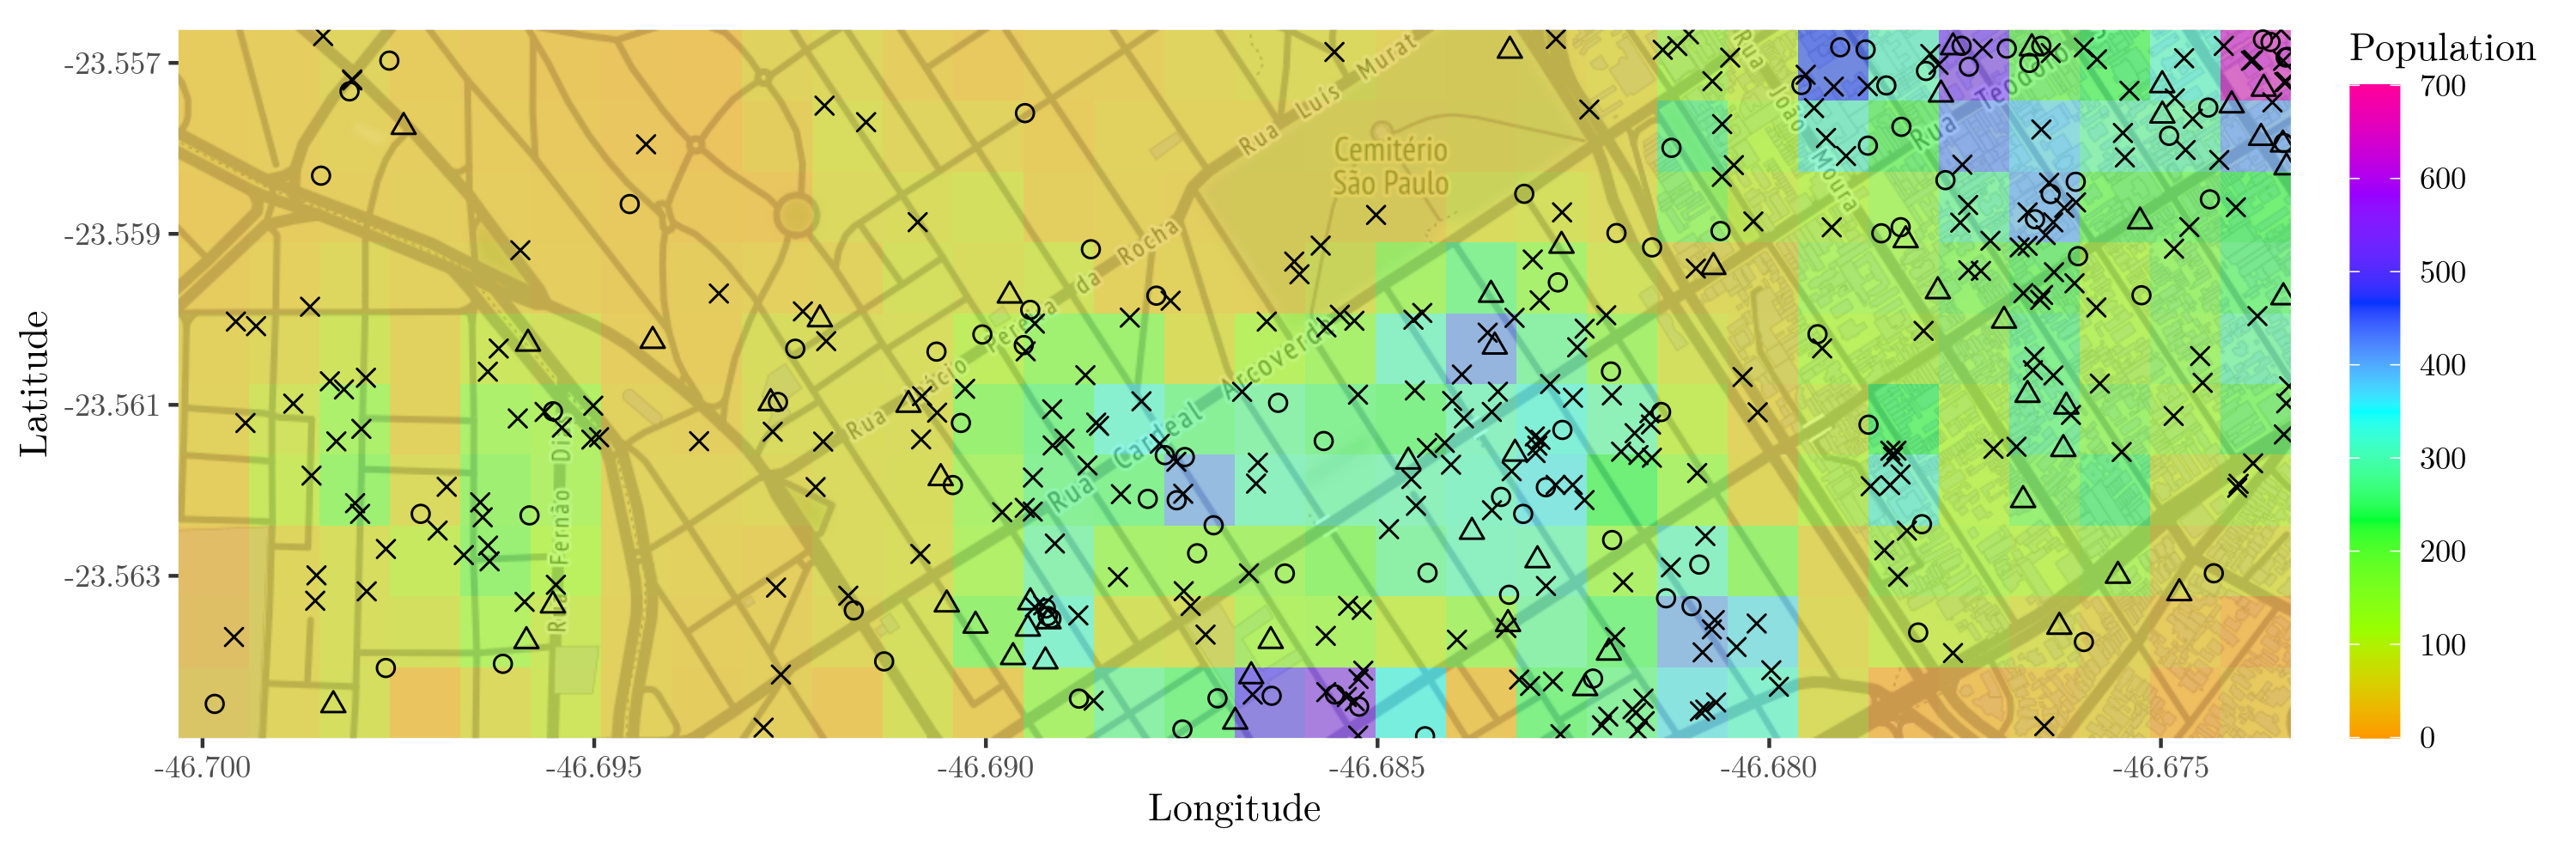
\includegraphics[width = 1\textwidth]{Images/map.png}\vspace{-12pt}
					\caption{\justifying São Paulo (Brazil) with the overlapped grid for the estimated population and infec. individuals' locations.}
					\label{fig:map}
				\end{figure}
			
				\vspace{-3pt}
			
				For two scenarios (\texttt{FC} and \texttt{EP}), we simulated the temporal curves and the spatio-temporal intensity functions. After fitting different models,
				\begin{figure}[!ht]
					\centering
					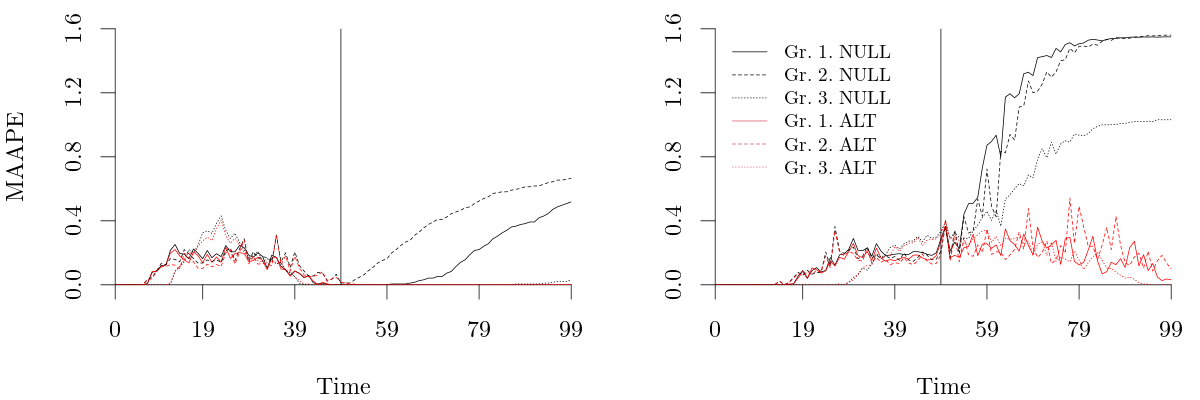
\includegraphics[width = 1\textwidth]{Images/computed_errors.png}\vspace{-6pt}
					\caption{\justifying Computed errors for groups 0--19, 20--59, 60+. Models were fitted with data up to $t_{49}$ (vertical solid line).}
					\label{fig:computederrors}
				\end{figure}
				
				\vspace{15pt}
				
				{\textcolor{strong-blue}{References}} \justifying \vspace{12pt} \tiny
				\bibliographystyle{plain}
				\bibliography{References/References}
				\end{block}	
							
			\end{column}
		
		\end{columns}
	\end{frame}


\end{document}